\documentclass{article}

% if you need to pass options to natbib, use, e.g.:
%     \PassOptionsToPackage{numbers, compress}{natbib}
% before loading neurips_2024


% ready for submission
% \usepackage{neurips_2024}


% to compile a preprint version, e.g., for submission to arXiv, add add the
% [preprint] option:
     \usepackage[preprint]{neurips_2024}


% to compile a camera-ready version, add the [final] option, e.g.:
%     \usepackage[final]{neurips_2024}


% to avoid loading the natbib package, add option nonatbib:
%    \usepackage[nonatbib]{neurips_2024}


\usepackage[utf8]{inputenc} % allow utf-8 input
\usepackage[T1]{fontenc}    % use 8-bit T1 fonts
\usepackage{hyperref}       % hyperlinks
\usepackage{url}            % simple URL typesetting
\usepackage{booktabs}       % professional-quality tables
\usepackage{amsfonts}       % blackboard math symbols
\usepackage{nicefrac}       % compact symbols for 1/2, etc.
\usepackage{microtype}      % microtypography
\usepackage{xcolor}         % colors
\usepackage{amsmath}
\usepackage{natbib}
\usepackage{graphicx}  % For including graphics
\usepackage{float}     % To control figure placement
\usepackage{geometry}
\usepackage{array}
\usepackage{multirow}
\usepackage{graphicx}
\usepackage{subcaption}



\title{Deep Learning 1 - Homework 3}


% The \author macro works with any number of authors. There are two commands
% used to separate the names and addresses of multiple authors: \And and \AND.
%
% Using \And between authors leaves it to LaTeX to determine where to break the
% lines. Using \AND forces a line break at that point. So, if LaTeX puts 3 of 4
% authors names on the first line, and the last on the second line, try using
% \AND instead of \And before the third author name.


\author{%
  Pedro M.P.~Curvo \\
  MSc Artificial Intelligence\\
  University of Amsterdam\\
  \texttt{pedro.pombeiro.curvo@student.uva.nl} \\
  % examples of more authors
  % \And
  % Coauthor \\
  % Affiliation \\
  % Address \\
  % \texttt{email} \\
  % \AND
  % Coauthor \\
  % Affiliation \\
  % Address \\
  % \texttt{email} \\
  % \And
  % Coauthor \\
  % Affiliation \\
  % Address \\
  % \texttt{email} \\
  % \And
  % Coauthor \\
  % Affiliation \\
  % Address \\
  % \texttt{email} \\
}


\begin{document}


\maketitle


% \begin{abstract}
%   The abstract paragraph should be indented \nicefrac{1}{2}~inch (3~picas) on
%   both the left- and right-hand margins. Use 10~point type, with a vertical
%   spacing (leading) of 11~points.  The word \textbf{Abstract} must be centered,
%   bold, and in point size 12. Two line spaces precede the abstract. The abstract
%   must be limited to one paragraph.
% \end{abstract}


\section*{Part 1}

\subsection*{1.1}

To sample an image using the decoder $f_{\theta}$ from the generative model described in this section, we first
need to sample a latent vector $z$ from the prior distribution $p(z)$. In this case, the prior distribution is a
standard multivariate Gaussian distribution, so we can sample $z$ from a standard normal distribution, i.e., $z \sim \mathcal{N}(0, I_D)$.

Then, we need to compute the pixel probabilities using the decoder $f_{\theta}$. For this, we pass
the sampled latent vector $z$ through the decoder $f_{\theta}$, which is a neural network parameterized by $\theta$.
This will map the latent vector $z$ to the probabilities of the Categorical distribution for each pixel $x_m$ in the image.
$f_{\theta}(z) \rightarrow (p_1, p_2, ..., p_k)^M$. 
Here: $p_m = (p_{m1}, p_{m2}, ..., p_{mk})$ are the event probabilities for pixel $m$ being in one of the $k$ categories. $M$ is the number of pixels in the image. 

Then, we can sample pixel values $x_n$ for each pixel $m$ by sampling from the Categorical distribution $Cat(x_m | f_{\theta}(z)_m)$, where, $x_m \sim Cat(p_m)$. This will generate the image by sampling each pixel value independently based on the probabilities computed by the decoder. 

Finally we combine the pixel values $x_m$ to from the image $x_n$. 

\subsection*{1.2}

% Monte Carlo integration with samples from $p(z_n)$ can be used to approximate the expectation of the log-likelihood. 
% However, is inefficient for training VAE models because it requires a large number of samples to accurately estimate the
% log-likelihood. This problem appears because the dimensionality of the latent space $z$ affects the number of samples
% needed to cover the entire latent space adequately. As the dimensionality of the latent space increases, the space
% becomes sparser, and more samples are needed to cover the space to capture the posterior distribution $p(z|x)$, which
% is often highly concentrated in certain regions of the latent space (as shown by the blue contours in Figure 2).

% This results in a exponentially increasing number of samples needed to accurately estimate the log-likelihood, 
% that is, $L \rightarrow \infty$ as $D \rightarrow \infty$. This makes Monte Carlo integration impractical for high-dimensional
% latent spaces due to the computational cost of sampling a large number of points to estimate the log-likelihood accurately.
% Therefore, other methods are used to estimate the log-likelihood in VAE models. 


Monte Carlo integration with samples from \( p(z_n) \) can approximate the expectation of the log-likelihood, but it is inefficient for training VAEs because it requires a large number of samples to achieve an accurate estimate. The inefficiency arises from the high-dimensional nature of the latent space \( z \).

As the dimensionality \( D \) of the latent space increases, the prior \( p(z) \) becomes increasingly sparse, and the true posterior \( p(z|x) \) often concentrates in specific regions of the latent space (illustrated by the blue contours in Figure 2). Consequently, a very large number of samples is required to adequately cover the latent space and accurately estimate the log-likelihood. This results in the computational cost scaling exponentially with the dimensionality of \( z \), making it impractical for high-dimensional latent spaces.

For this reason, VAEs use an alternative approach, such as the variational posterior \( q(z|x) \), which focuses sampling in regions of high posterior density, improving efficiency and scalability.



\newpage
\subsection*{1.3}

From Equation 10, we have:

\begin{align*}
    \log p(x_n) - KL(q_{\theta}(z_n|x_n) || p(z_n|x_n)) &= \mathbb{E}_{q_{\theta}(z_n|x_n)}[\log p(x_n|z_n)] - KL(q_{\theta}(z_n|x_n) || p(z_n)) \\
\end{align*}

Rearranging the equation we get: 

\begin{align*}
    \log p(x_n) &= \mathbb{E}_{q_{\theta}(z_n|x_n)}[\log p(x_n|z_n)] - KL(q_{\theta}(z_n|x_n) || p(z_n)) + KL(q_{\theta}(z_n|x_n) || p(z_n|x_n)) \\
\end{align*}

Now, we know the KL divergence is always non-negative, since it is a measure of the difference between two distributions by
measuring how much one probability distribution diverges from a second, expected probability distribution. It is zero if and only if the two distributions are the same.
Mathematically, we have that: 

\begin{align*}
    KL(q_{\theta}(z_n|x_n) || p(z_n)) &\geq 0 \\
    KL(q_{\theta}(z_n|x_n) || p(z_n|x_n)) &\geq 0 \\
\end{align*}

With this we have that: 

\begin{align*}
  \log p(x_n) &= \mathbb{E}_{q_{\theta}(z_n|x_n)}[\log p(x_n|z_n)] - KL(q_{\theta}(z_n|x_n) || p(z_n)) + KL(q_{\theta}(z_n|x_n) || p(z_n|x_n)) \\
  &\geq \mathbb{E}_{q_{\theta}(z_n|x_n)}[\log p(x_n|z_n)] - KL(q_{\theta}(z_n|x_n) || p(z_n)) \\
\end{align*}

Therefore, the right-hand side of the equation $\mathbb{E}_{q_{\theta}(z_n|x_n)}[\log p(x_n|z_n)] - KL(q_{\theta}(z_n|x_n) || p(z_n))$ is
always less than or equal to the true log-likelihood $\log p(x_n)$. Hence, the right-hand side of the equation is a lower bound on the true log-likelihood.

\newpage
\subsection*{1.4}

ELBO consists of two terms: 

\begin{align*}
    ELBO(x_n) &= \mathbb{E}_{q_{\theta}(z_n|x_n)}[\log p(x_n|z_n)] - KL(q_{\theta}(z_n|x_n) || p(z_n)) \\
\end{align*}

The first term, $\mathbb{E}_{q_{\theta}(z_n|x_n)}[\log p(x_n|z_n)]$, represents the expected log-likelihood of the data $x_n$ given the latent variable $z_n$.
However, this value stays the same regardless of how $q(z_n|x_n)$ is chosen.
The second term, $KL(q_{\theta}(z_n|x_n) || p(z_n))$, represents the KL divergence between the approximate posterior $q_{\theta}(z_n|x_n)$ and the prior $p(z_n)$.
As $q_{\theta}(z_n|x_n)$ approaches the true posterior $p(z_n|x_n)$, the KL divergence term decreases towards zero. This
is because the KL divergence is minimized when the two distributions are the same, $q(z_n|x_n) = p(z_n|x_n)$.
With that being said, as the KL divergence term decreases, the ELBO increases. becoming closer to the true log-likelihood $\log p(x_n)$.
Ideally, when $q(z_n|x_n) = p(z_n|x_n)$, the ELBO is equal to the true log-likelihood $\log p(x_n)$.

So: 

\begin{align*}
    \lim_{q_{\theta}(z_n|x_n) \rightarrow p(z_n|x_n)} ELBO(x_n) &= \lim_{q_{\theta}(z_n|x_n) \rightarrow p(z_n|x_n)} \mathbb{E}_{q_{\theta}(z_n|x_n)}[\log p(x_n|z_n)] - KL(q_{\theta}(z_n|x_n) || p(z_n)) \\
    &= \mathbb{E}_{p(z_n|x_n)}[\log p(x_n|z_n)] - \lim_{q_{\theta}(z_n|x_n) \rightarrow p(z_n|x_n)} KL(q_{\theta}(z_n|x_n) || p(z_n)) \\
    &= \mathbb{E}_{p(z_n|x_n)}[\log p(x_n|z_n)] - KL(p(z_n|x_n) || p(z_n)) \\
    &= \mathbb{E}_{p(z_n|x_n)}[\log p(x_n|z_n)] - 0 \\
    &= \mathbb{E}_{p(z_n|x_n)}[\log p(x_n|z_n)] \\
    &= \log p(x_n) \\
\end{align*}

And that is why the main goal of training a VAE is to maximize the ELBO, as it is a lower bound on the true log-likelihood $\log p(x_n)$.
And this corresponds to minimizing the KL divergence between the approximate posterior $q_{\theta}(z_n|x_n)$ and the prior $p(z_n)$.

\subsection*{1.5}

The names \textbf{reconstruction} loss and \textbf{regularization} loss are used because: 

\begin{itemize}
  \item \textbf{Reconstruction Loss}: The term $\mathbb{E}_{q_{\theta}(z_n|x_n)}[\log p(x_n|z_n)]$ is the expected log-likelihood
  of the data $x_n$ given the latent variable $z_n$. Hence, it is a measure of how well the model can reconstruct the
  observed data $x_n$ from the latent variable $z_n$. Meaning, it directly corresponds to the task of reconstructing the
  original input, being the main objective of the model. Therefore, it is called the \textbf{reconstruction} loss.

  \item\textbf{Regularization Loss:} The term $KL(q_{\theta}(z_n|x_n) || p(z_n))$ is the KL divergence and ensures
that the learned posterior distribution $q_{\theta}(z_n|x_n)$ is close to the prior distribution $p(z_n)$. This term
regularizes the model by preventing the posterior distribution from deviating too much from the prior distribution.
Therefore, it is called the \textbf{regularization} loss.
\end{itemize}

\newpage

\subsection*{1.6}

When the prior distribution $p(z_n)$ and variational posterior $q_{\theta}(z_n|x_n)$ are not Gaussian, the KL divergence
term $KL(q_{\theta}(z_n|x_n) || p(z_n))$ cannot be computed simply in closed form. To overcome this, we can use the
Monte Carlo approximation to estimate the regularization term. 

The regularization term in the VAE is the KL divergence between the variational distribution $q_{\theta}(z_n|x_n)$ and the prior distribution $p(z_n)$.
Mathematically, this term is defined as:
\begin{align*}
    D_{KL}(q_{\theta}(z_n|x_n) || p(z_n)) &= \mathbb{E}_{q_{\theta}(z_n|x_n)}[\log \frac{q_{\theta}(z_n|x_n)}{p(z_n)}] \\
\end{align*}
Assuming the closed-form expression for the KL divergence is intractable, we can use the Monte Carlo approximation to estimate the KL divergence.
First, we sample $L$ latent vectors $z_n^{(l)}$ from the variational distribution $q_{\theta}(z_n|x_n)$, where $l = 1, 2, ..., L$.
Then, we compute the log-ratio of the variational distribution and the prior distribution for each sample:
\begin{align*}
    \log \frac{q_{\theta}(z_n^{(l)}|x_n)}{p(z_n)} \\
\end{align*}
where $q_{\theta}(z_n^{(l)}|x_n)$ is the probability density of the variational distribution evaluated at the sample $z_n^{(l)}$.
Finally, we compute the Monte Carlo estimate of the KL divergence as:

\begin{align*}
    D_{KL}(q_{\theta}(z_n|x_n) || p(z_n)) &\approx \frac{1}{L} \sum_{l=1}^{L} \log \frac{q_{\theta}(z_n^{(l)}|x_n)}{p(z_n)} \\
\end{align*}
Then, we can use this approximation in the loss function:
\begin{align*}
    \mathbb{L}_{regularization,n} &\approx \frac{1}{L} \sum_{l=1}^{L} \log \frac{q_{\theta}(z_n^{(l)}|x_n)}{p(z_n)} \\
\end{align*}
This methods allows us to estimate the KL divergence term when the prior and variational posterior are not Gaussian. The more
samples we use, the more accurate the estimate will be, but it will also increase the computational cost of training the model.
This method can be used for any arbitrary prior and variational posterior distributions, as long as we can sample from the variational distribution
and compute the log-ratio of the two distributions.

It is important to note that in this case, sampling from \( q_{\theta}(z_n|x_n) \) is significantly more efficient than using Monte Carlo integration to estimate the log-likelihood by sampling directly from \( p(z_n) \). Sampling from the prior distribution \( p(z_n) \) can be inefficient because the prior may not accurately capture the structure of the data. As a result, many samples may be drawn from regions in the latent space \( z_n \) that contribute little or nothing to \( p(x_n | z_n) \), leading to a poor estimate of the log-likelihood. For instance, when \( p(z_n) \) is a standard normal distribution, it spans the entire latent space, whereas the posterior distribution \( p(z_n | x_n) \) is typically concentrated in specific regions of the latent space, as illustrated by the blue contours in the image.

By contrast, sampling from the variational distribution \( q_{\theta}(z_n|x_n) \) is much more effective. This distribution is designed to approximate the true posterior \( p(z_n | x_n) \), and as such, it focuses sampling on the regions of the latent space that are most relevant to the data. Samples drawn from \( q_{\theta}(z_n|x_n) \) are concentrated in areas where the posterior is high, meaning they are more likely to contribute meaningfully to the log-likelihood estimate. This targeted sampling reduces the number of samples needed for accurate estimation, making Monte Carlo integration more efficient. In other words, leveraging \( q_{\theta}(z_n|x_n) \) as the sampling distribution ensures that computational resources are focused on regions of the latent space that matter most, leading to better performance and efficiency.


\subsection*{1.7}

When sampling directly from a distribution \( q_{\theta}(z_n|x_n) \) to estimate the expectation \( \mathbb{E}_{q_{\theta}(z_n|x_n)}[\log p(x_n|z_n)] \), the sampling process itself is non-differentiable with respect to the parameters \( \theta \). This is because sampling introduces randomness that disrupts the smooth computation graph required for gradient-based optimization. As a result, the gradients of the loss function with respect to the encoder parameters \( \theta \) cannot be computed directly using standard backpropagation.

The \textbf{reparameterization trick} resolves this issue by making the sampling process differentiable. Instead of sampling \( z_n \) directly from \( \mathcal{N}(\mu_{\theta}(x_n), \Sigma_{\theta}(x_n)) \), the random variable \( z_n \) is reparameterized as a deterministic transformation of a noise variable \( \epsilon \sim \mathcal{N}(0, I_D) \). Specifically, \( z_n \) is expressed as:

\begin{align*}
    z_n = \mu_{\theta}(x_n) + \sigma_{\theta}(x_n) \odot \epsilon
\end{align*}
where \( \mu_{\theta}(x_n) \) and \( \sigma_{\theta}(x_n) \) are the encoder outputs parameterized by \( \theta \), and \( \odot \) denotes element-wise multiplication. 

This reformulation ensures that the randomness is isolated in \( \epsilon \), which is independent of \( \theta \). Consequently, the sampling operation becomes differentiable with respect to \( \theta \), allowing gradients of the loss function to propagate through the encoder network via backpropagation.


\newpage
\subsection*{1.8}

\begin{table}[h]
    \centering
    \begin{tabular}{|c|}
    \hline
    \textbf{Test BPD} \\
    \hline
    0.518 \\
    \hline
    \end{tabular}
\end{table}

\begin{figure}[h]
    \centering
    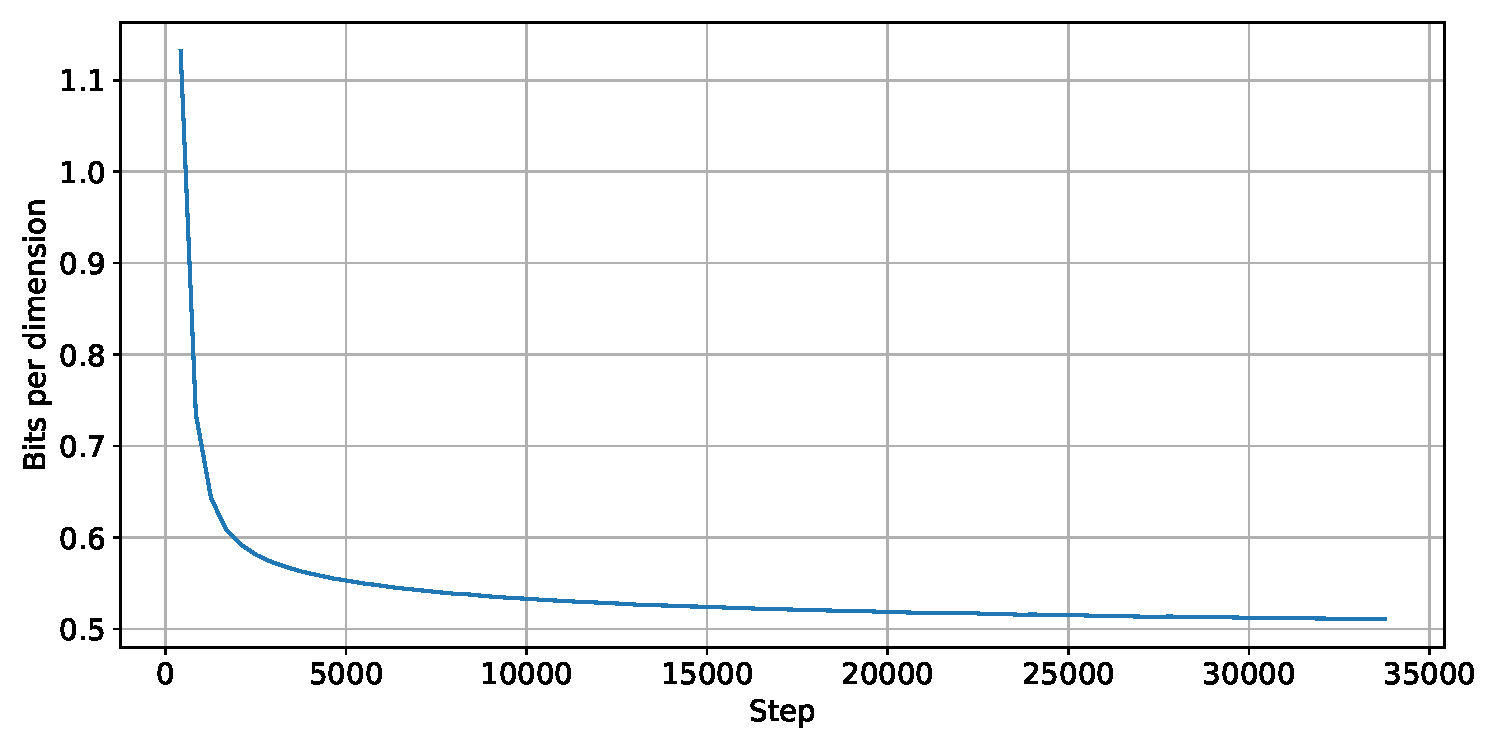
\includegraphics[width=\textwidth]{images/train_bpd.pdf}
    \caption{Train BPD for VAE with latent dim=20}
    \label{fig:train_bpd}
\end{figure}
\begin{figure}
    \centering
    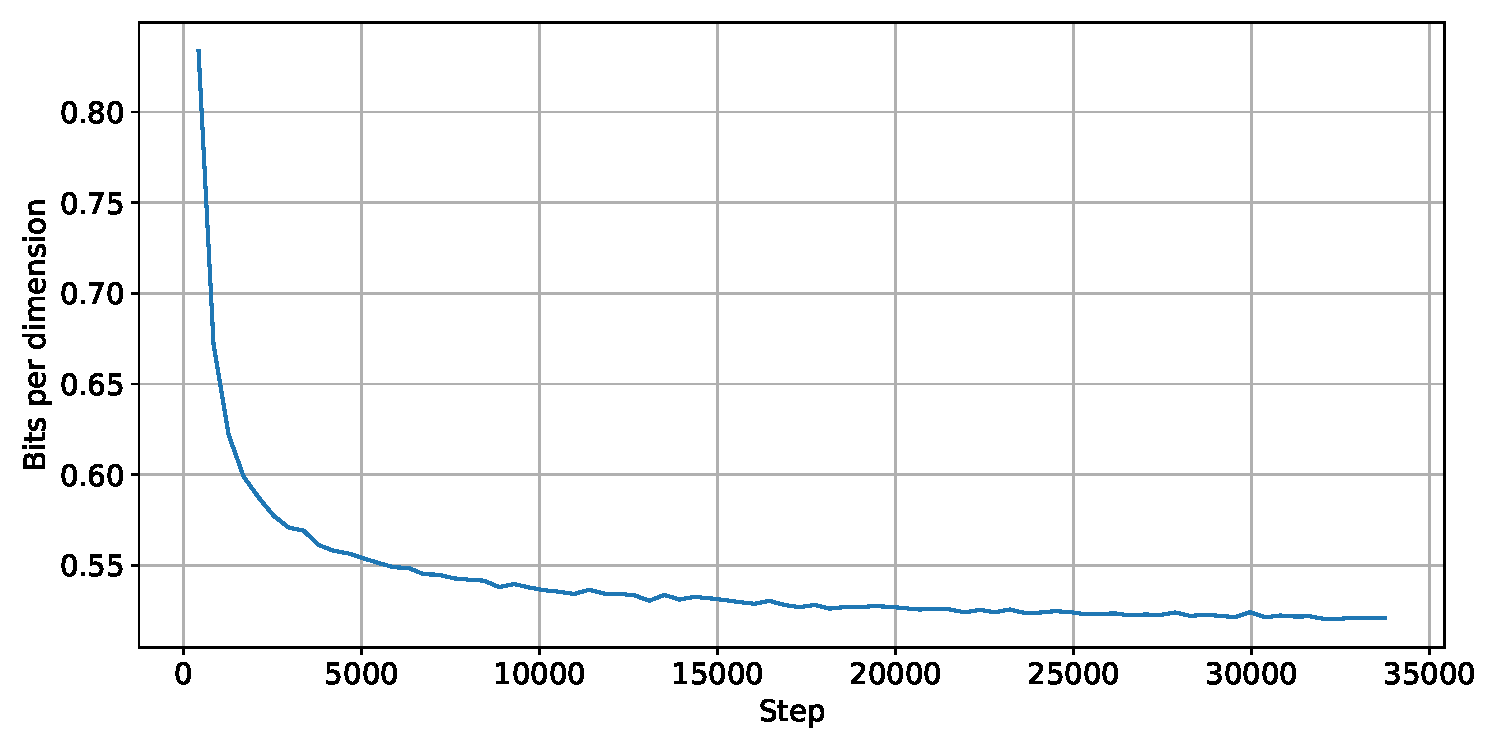
\includegraphics[width=\textwidth]{images/val_bpd.pdf}
    \caption{Validation BPD for VAE with latent dim=20}
    \label{fig:val_bpd}
\end{figure}

\subsection*{1.9}

\begin{figure}[H]
    \centering
    \begin{minipage}{0.3\textwidth}
        \centering
        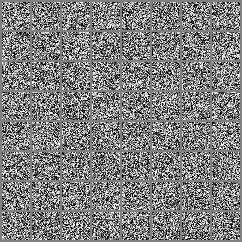
\includegraphics[width=\textwidth]{images/epoch_0_samples.png}
        \caption{Epoch 0}
        \label{fig:epoch_0}
    \end{minipage}
    \hfill
    \begin{minipage}{0.3\textwidth}
        \centering
        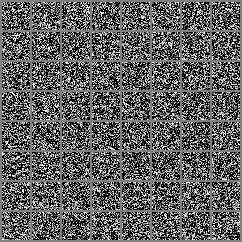
\includegraphics[width=\textwidth]{images/epoch_10_samples.png}
        \caption{Epoch 10}
        \label{fig:epoch_10}
    \end{minipage}
    \hfill
    \begin{minipage}{0.3\textwidth}
        \centering
        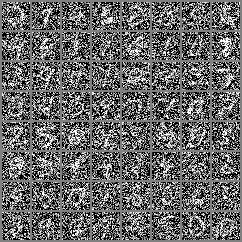
\includegraphics[width=\textwidth]{images/epoch_80_samples.png}
        \caption{Epoch 80}
        \label{fig:epoch_80}
    \end{minipage}
    \caption{Visualization of the VAE training progress at epochs 0, 10, and 80.}
    \label{fig:vae_epochs}
\end{figure}

By looking at the images generated by the VAE model before training, middle of training, and after training, we can see that initially we only have noise in the images, as the model has not learned to generate meaningful images yet. As the model trains, the images start to become more recognizable, and we start to see some numbers appearing in the images resembling the digits in the MNIST dataset, but with some imperfections. At the end of training, I see that the images are more refined and resemble the digits in the MNIST dataset more closely, with fewer imperfections and noise, showing the model has learned to generate more accurate and realistic images as it trains.

\subsection*{1.10}

% Manifold image 

% Manifold image 
\begin{figure}[H]
    \centering
    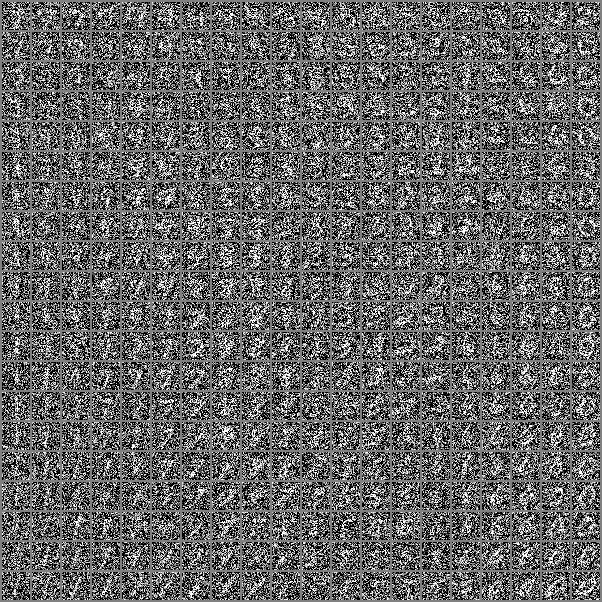
\includegraphics[width=0.8\textwidth]{images/vae_manifold.png}
    \caption{Visualization of the data manifold learned by the VAE. The manifold shows the reconstructed images from the
    2-dimensional latent space.}
    \label{fig:vae_manifold}
\end{figure}

The manifold illustrates the latent space learned by the VAE, decoded into MNIST digits. Points in the latent space that correspond to similar digits seemed to be grouped into clusters, occupying distinct regions in the grid. This clustering shows that the VAE encodes similar digits closer together in the latent space. For example, digits that are visually alike are positioned near each other, resulting in smooth transitions between neighboring points.

Some areas contain blurry or incomplete digits, indicating regions where the model struggles to represent the data distribution accurately, specially in the boundaries between different digits.


\newpage
\section*{Part 2}

\subsection*{2.1}

% Table with arguments 
\begin{table}[h!]
    \centering
    \begin{tabular}{|c|c|c|c|c|c|c|}
    \hline
    \textbf{Argument} & \textbf{batch\_size} & \textbf{valid\_ratio} & \textbf{augmentations} & \textbf{pretrained} & \textbf{num\_epochs} & \textbf{train\_strats} \\
    \hline
    \textbf{Value} & 64 & 0.75 & False & True & 30 & ['standard'] \\
    \hline
    \textbf{Argument} & \textbf{visualise} & \textbf{epsilon\_fgsm} & \textbf{alpha\_fgsm} & \textbf{epsilon\_pgd} & \textbf{alpha\_pgd} & \textbf{num\_iter\_pgd} \\
    \hline
    \textbf{Value} & True & 0.1 & 0.5 & 0.01 & 2 & 10 \\
    \hline
    \end{tabular}
    \caption{Configuration used for a pretrained ResNet18 with and without FGSM attack}
\end{table}

\begin{table}[h!]
    \centering
    \begin{tabular}{|c|c|c|}
    \hline
    \textbf{Attack Test Type} & \textbf{Parameters} & \textbf{Test Accuracy} \\
    \hline
    Without & - & 0.93 \\
    \hline
    FGSM & Alpha: 0.5, Epsilon: 0.1 & 0.41 \\
    \hline
    PGD & Alpha: 2, Epsilon: 0.01, Num Iter: 10 & 0.4228 \\
    \hline
    \end{tabular}
    \caption{Testing results for \textbf{standard} training loss for different attacks using a \textbf{pretrained} ResNet18}
\end{table}



\begin{itemize}
    \item \textbf{i)} Adding a random perturbation of size $\epsilon$ does not target the specific vulnerability of the model, but rather adds noise to the input data. FGSM, on the other hand, is a targeted attack, since it uses the gradient of the loss function to find the direction in which the input data should be perturbed to maximize the loss for a given input. This targeted attack is more effective at fooling the model than adding random noise. It also ensures that the perturbation aligns with the model decision boundary, making it more likely to fool the model. Random noise, on the other hand, is unlikely to align with the decision boundary, making it less effective at fooling the model.

    \item \textbf{ii)} This phenomenon occurs because both models A and B, despite being trained on different subsets of the data, are optimized for the same task and learn to extract similar features from the data. As a result, they develop similar high-level representations and decision boundaries. Adversarial perturbations exploit weaknesses in these representations by pushing inputs in directions that maximize the loss, perturbation that align with the models' decision boundary (and in this case A and B will have similar decision boundaries). These directions often correspond to vulnerabilities shared by both models due to the shared structure of the data and the shared task.

    In high-dimensional spaces, even small perturbations designed for one model are likely to remain effective on another one because of the inherent similarities in their learned feature spaces and gradients. This shared susceptibility leads to the transferability of adversarial examples between models trained for the same task.

    \item \textbf{iii)} Models trained with data augmentation are more robust to adversarial examples because data augmentation introduces noise and perturbations to the training data, which makes the model more robust to small perturbations in the input. When the model is trained with augmented data, such as adding noise, rotations, or translations to the training images, the model learns to generalize better and consequently the model's decision boundary becomes smoother and less sensitive and reactive to small, targeted perturbations. This makes it harder for an attacker to generate adversarial examples that fool the model.
\end{itemize}

\subsection*{2.2}

\begin{table}[H]
    \centering
    \begin{tabular}{|c|cccccc|}
    \hline
    \textbf{Argument} & \multicolumn{6}{|c|}{\textbf{Values}} \\
    \hline
    batch\_size &       \multicolumn{6}{c|}{64} \\
    valid\_ratio &      \multicolumn{6}{c|}{0.75} \\
    num\_epochs &       \multicolumn{6}{c|}{30} \\
    epsilon\_fgsm &     \multicolumn{6}{c|}{0.1} \\
    alpha\_fgsm &       \multicolumn{6}{c|}{0.5} \\
    epsilon\_pgd &      \multicolumn{6}{c|}{0.01} \\
    alpha\_pgd &        \multicolumn{6}{c|}{2} \\
    num\_iter\_pgd &    \multicolumn{6}{c|}{10} \\
    visualise &         \multicolumn{6}{c|}{True} \\
    Device &            \multicolumn{6}{c|}{GPU} \\
    augmentations & \textbf{-}  & \textbf{False} & \textbf{False} & \textbf{True} & \textbf{False} & \textbf{True} \\
    pretrained & \textbf{True}  & \textbf{False} & \textbf{False} & \textbf{True} & \textbf{False} & \textbf{False}\\
    train\_strats & [standard] & [standard] & [fgsm] & [fgsm] & [pgd] & [pgd]\\
    \hline
    Attack & \multicolumn{6}{c|}{\textbf{Test Accuracy}}\\
    \hline
    Without     & 93.00\% & 67.00\% & 61.00\% & 87.00\% & 53.00\% & \\
    FGSM        & 41.00\% & 17.36\% & 23.20\% & 56.24\% & 30.32\% & \\
    PGD         & 42.48\% & 15.88\% & 24.52\% & 62.24\% & 25.32\% & \\
    \hline
    \multicolumn{7}{|c|}{\textbf{}}\\
    \hline
    Train Loss                  & & 0.2033 & 1.0450 & 0.2839 & 0.6887 & \\
    Train Accuracy              & & 0.9548 & 0.7514 & 0.9949 & 0.7705 & \\
    Validation Loss             & & 0.9880 & 1.0957 & 0.3586 & 1.7670 & \\
    Validation Accuracy         & & 0.6694 & 0.6103 & 0.8810 & 0.5058 & \\
    Best Validation Accuracy    & & 0.6727 & 0.6171 & 0.8859 & 0.5373 & \\
    \hline
    \end{tabular}
    \caption{Trained models (the columns that matter to this question are the second and third where we can see the results for with/without defense and with/without attacks)\textbf{ Note:} We observe that by using a pretrained model and then using augmentation we get the best accuracy. This might be since we are finetunning the model with the adversial augmentation.}
\end{table}

% \begin{table}[H]
%     \centering
%     \begin{tabular}{|c|c|}
%     \hline
%     \textbf{Metric} & \textbf{Value} \\
%     \hline
%     \textbf{Train Loss} & 0.9781 \\
%     \textbf{Train Accuracy} & 0.7701 \\
%     \hline
%     \textbf{Validation Loss} & 1.0832 \\
%     \textbf{Validation Accuracy} & 0.6115 \\
%     \hline
%     \textbf{Training Time} & 8m 53s \\
%     \hline
%     \textbf{Best Validation Accuracy} & 0.618644 \\
%     \hline
%     \textbf{Test Accuracy} & 62\% \\
%     \hline
%     \multicolumn{2}{|c|}{\textbf{FGSM Attack}} \\
%     \hline
%     \textbf{Args} & \{'alpha': 0.5, 'epsilon': 0.1\} \\
%     \textbf{Test Accuracy} & 0.2584 \\
%     \hline
%     \end{tabular}
%     \caption{Model Performance and Adversarial Attack Results for FGSM loss without Defense}
% \end{table}

% \begin{table}[H]
%     \centering
%     \begin{tabular}{|c|c|}
%     \hline
%     \textbf{Metric} & \textbf{Value} \\
%     \hline
%     \textbf{Train Loss} & 1.0450 \\
%     \textbf{Train Accuracy} & 0.7514 \\
%     \hline
%     \textbf{Validation Loss} & 1.0957 \\
%     \textbf{Validation Accuracy} & 0.6103 \\
%     \hline
%     \textbf{Training Time} & 8m 55s \\
%     \hline
%     \textbf{Best Validation Accuracy} & 0.617055 \\
%     \hline
%     \textbf{Test Accuracy} & 61\% \\
%     \hline
%     \multicolumn{2}{|c|}{\textbf{Adversarial Attacks}} \\
%     \hline
%     \textbf{FGSM Args} & \{'alpha': 0.5, 'epsilon': 0.1\} \\
%     \textbf{FGSM Test Accuracy} & 0.232 \\
%     \hline
%     \textbf{PGD Args} & \{'alpha': 2, 'epsilon': 0.01, 'num\_iter': 10\} \\
%     \textbf{PGD Test Accuracy} & 0.2452 \\
%     \hline
%     \end{tabular}
%     \caption{Model Training and Adversarial Attack Results for FGSM loss with defense}
% \end{table}

% \begin{table}[H]
%     \centering
%     \begin{tabular}{|c|c|}
%     \hline
%     \textbf{Metric} & \textbf{Value} \\
%     \hline
%     \textbf{Train Loss} & 0.2837 \\
%     \textbf{Train Accuracy} & 0.9949 \\
%     \hline
%     \textbf{Validation Loss} & 0.4018 \\
%     \textbf{Validation Accuracy} & 0.8705 \\
%     \hline
%     \textbf{Training Time} & 8m 53s \\
%     \hline
%     \textbf{Best Validation Accuracy} & 0.880826 \\
%     \hline
%     \textbf{Test Accuracy} & 88\% \\
%     \hline
%     \multicolumn{2}{|c|}{\textbf{Adversarial Attacks}} \\
%     \hline
%     \textbf{FGSM Args} & \{'alpha': 0.5, 'epsilon': 0.1\} \\
%     \textbf{FGSM Test Accuracy} & 0.4988 \\
%     \hline
%     \end{tabular}
%     \caption{Model Training and Adversarial Attack Results for FGSM loss without defense using pretrained and augmentation}
% \end{table}

% \begin{table}[H]
%     \centering
%     \begin{tabular}{|c|c|}
%     \hline
%     \textbf{Metric} & \textbf{Value} \\
%     \hline
%     \textbf{Train Loss} & 0.2839 \\
%     \textbf{Train Accuracy} & 0.9949 \\
%     \hline
%     \textbf{Validation Loss} & 0.3586 \\
%     \textbf{Validation Accuracy} & 0.8810 \\
%     \hline
%     \textbf{Training Time} & 8m 51s \\
%     \hline
%     \textbf{Best Validation Accuracy} & 0.885858 \\
%     \hline
%     \textbf{Test Accuracy} & 87\% \\
%     \hline
%     \multicolumn{2}{|c|}{\textbf{Adversarial Attacks}} \\
%     \hline
%     \textbf{FGSM Args} & \{'alpha': 0.5, 'epsilon': 0.1\} \\
%     \textbf{FGSM Test Accuracy} & 0.5624 \\
%     \hline
%     \textbf{PGD Args} & \{'alpha': 2, 'epsilon': 0.01, 'num\_iter': 10\} \\
%     \textbf{PGD Test Accuracy} & 0.6224 \\
%     \hline
%     \end{tabular}
%     \caption{Model Training and Adversarial Attack Results for FGSM loss with defense, pretrained and augmentation}
% \end{table}

Without defense the model focuses solely on minimizing the loss on clean data, leading to high accuracy on natural,
unperturbed inputs. However, it remains highly vulnerable to adversarial attacks, as it lacks mechanisms to handle small, targeted perturbations. That's why we see that without an attack we get 67\% accuracy, but with FGSM we get 17\%.

With defense, the model gains robustness to adversarial attacks by incorporating adversarial training. With this,
the model learns smoother decision boundaries and learns how to adapt to small perturbations in the input data. This
can reduce its accuracy on clean data (we see a drop to 61\%) because the model shifts its focus from purely optimizing performance on the clean dataset to balancing performance on both clean and adversarial examples. This can lead to a decrease in accuracy on clean data. Hence, the models with defense often sacrifice better generalization on clean data to gain robustness to adversarial attacks (we observe better accuracy on adversarial attack - 23\% compared to without defense).

This trade-off occurs because neural networks have \textbf{limited capacity} and must allocate resources to learn to generalize.
Allocating some of this capacity to handle adversarial perturbations reduces the focus on patterns in clean data, leading to a decrease in accuracy on clean data.
Besides this, defending against adversarial attacks often involves smoothing or reshaping decision boundaries to make them robust to perturbations, However, this might \textbf{oversimplify the boundary}, causing the model to misclassify some clean data points.
During adversarial training, it might also be possible that the model might overfit to specific types of adversarial perturbations, as the FGSM, reducing the accuracy on clean data.


\newpage
\subsection*{2.3}

\begin{table}[H]
    \centering
    \begin{tabular}{|c|ccccccc|}
    \hline
    \textbf{Argument} & \multicolumn{7}{|c|}{\textbf{Values}} \\
    \hline
    batch\_size &       \multicolumn{7}{c|}{64} \\
    valid\_ratio &      \multicolumn{7}{c|}{0.75} \\
    num\_epochs &       \multicolumn{7}{c|}{30} \\
    epsilon\_fgsm &     \multicolumn{7}{c|}{0.1} \\
    alpha\_fgsm &       \multicolumn{7}{c|}{0.5} \\
    epsilon\_pgd &      \multicolumn{7}{c|}{0.01} \\
    alpha\_pgd &        \multicolumn{7}{c|}{2} \\
    num\_iter\_pgd &    \multicolumn{7}{c|}{10} \\
    visualise &         \multicolumn{7}{c|}{True} \\
    Device &            \multicolumn{7}{c|}{GPU} \\
    augmentations & \textbf{-}  & \textbf{False} & \textbf{False} & \textbf{True} & \textbf{False} & \textbf{True} & \textbf{True}\\
    pretrained & \textbf{True}  & \textbf{False} & \textbf{False} & \textbf{True} & \textbf{False} & \textbf{False}& \textbf{True}\\
    train\_strats & [standard] & [standard] & [fgsm] & [fgsm] & [pgd] & [pgd] & [pgd] \\
    \hline
    Attack & \multicolumn{7}{c|}{\textbf{Test Accuracy}}\\
    \hline
    Without     & 93.00\% & 67.00\% & 61.00\% & 87.00\% & 53.00\% & 50.00\% & 86.00\% \\
    FGSM        & 41.00\% & 17.36\% & 23.20\% & 56.24\% & 30.32\% & 29.08\% & 59.36\% \\
    PGD         & 42.48\% & 15.88\% & 24.52\% & 62.24\% & 25.32\% & 29.12\% & 69.52\%\\
    \hline
    \multicolumn{8}{|c|}{\textbf{}}\\
    \hline
    Train Loss                  & & 0.2033 & 1.0450 & 0.2839 & 0.6887 &1.1393 &0.1748 \\
    Train Accuracy              & & 0.9548 & 0.7514 & 0.9949 & 0.7705 &0.5918 &0.9392 \\
    Validation Loss             & & 0.9880 & 1.0957 & 0.3586 & 1.7670 &1.6361 & 0.5664 \\
    Validation Accuracy         & & 0.6694 & 0.6103 & 0.8810 & 0.5058 &0.4845 & 0.8502 \\
    Best Validation Accuracy    & & 0.6727 & 0.6171 & 0.8859 & 0.5373 &0.5173 &0.8712 \\
    \hline
    \end{tabular}
    \caption{Trained models}
\end{table}

We observe that with pgd we get a better accuracy than with fgsm in adversarial attacks, but we loose overall accuracy wihtout any attacks, which is expected since PGD applies an iterative approach and can find more effective adversarial examples than FGSM. We also observe that the model trained with augmentation performs better (in attacks) than its counterpart without augmentation, which is expected as augmentation helps the model generalize better and become more robust to adversarial attacks.

\subsubsection*{i)}

Comparing adversarial loss and adding adversarial examples to the batch: 

\begin{itemize}
    \item \textbf{Adversarial loss}: Adversarial loss incorporates adversarial examples directly into the objective function. This is done by adding adversarial perturbations to the loss term, mixing clean and adversarial gradients during each training step. This approach allows the model to learn from adversarial examples during the forward pass while still using the original input for calculating the primary loss. This method is efficient and straightforward, since it integrates adversarial examples directly into the loss function. It also separates the clean and adversarial data by using distinct loss terms for each. This separation can help prevent overfitting/underfitiing to adversarial perturbations, as the overall loss is a combination of clean and adversarial components. By smoothing one, the other may remain unaffected, preserving a balanced loss landscape. However, implementing adversarial loss requires modifying the loss function, which can lead to more finetunning. 

    \item \textbf{Adding adversarial examples to the batch}: In this approach, the adversarial examples are explicitly
    generated and added to the batch during training, along with the original clean and samples. This results in the model training on a larger batch that contains both clean and adversarial examples, forcing the model to correctly classify  both types of examples. It has the pros of the model seeing both types of inputs (clean and adversarial) in each iteration, increasing robustness. It has the cons of an increasing computational cost, because we are increasing the batch size. Besides that, since we are now using the same loss function for both clean and adversarial examples, the model might overfit to the adversarial examples leading to a decrease in accuracy on clean data or oversmoothing the loss landscape (which now is just one overall), hurting the model's performance on clean data.
\end{itemize}

\textbf{Difference:} The key difference is that the adversarial loss modifies the optimization process directly by changing the objective function, while adding adversarial examples to the batch increases the diversity of the training data.

\textbf{Alignment:} These two methods may align when the adversarial loss function effectively integrates perturbations in a manner similar to how adversarial examples are added to the batch. 

\textbf{Divergence:} They could diverge in scenarios where the adversarial loss focuses more on optimizing the network's response to perturbations, while adding adversarial examples to the batch gives the model a broader exposure to such attacks without necessarily optimizing its response to them directly. Adversarial loss is computationally more efficient, while batch augmentation demands greater resources due to increased batch sizes.

\subsubsection*{ii)}

One advantage of the FGSM is the \textbf{speed}. FGSM is a single-step attack that computes the gradient once and adds a small perturbation based on that, making it very fast and computationally efficient compared to iterative attacks. However, its \textbf{effectiveness} is a limitation. FGSM produces more noticeable perturbations because it only takes a single step, and the model is more likely to recognize the pattern of the perturbation.

The PGD has the advantage of \textbf{robustness}. PGD is an iterative process which computes small gradient-based steps and projects the perturbed data back within the allowable $\epsilon$-ball. This allows it to find more effective adversarial examples that are harder for the model to detect and often less perceptible to human observers. However, its disadvantage is being \textbf{slower}. The iterative nature makes it computationally expensive and significantly slower than FGSM.

The overall trade-off between FGSM and PGD depends on the specific use case and requirements, that is, \textbf{Speed vs Robustness}. FGSM is faster and computationally less demanding, making it suitable for quick attacks or scenarios where computational resources are limited. However, it is less effective than PGD in generating adversarial examples that cause consistent misclassifications, resulting in lower robustness to adversarial examples.

PGD is computationally more expensive due to its iterative nature but generates more precise adversarial examples that are harder for the model to classify correctly. This makes it more effective at improving a model's robustness to adversarial attacks.





















\newpage
\bibliographystyle{abbrvnat}
\bibliography{references} 


\end{document}